\documentclass[11pt]{article}
\usepackage{amsfonts}
\usepackage{amsmath}
\usepackage{amsthm}
\usepackage{amssymb}
\usepackage{mathrsfs}
\usepackage[fit]{truncate}
\usepackage{acl2012}
\usepackage{times}
\usepackage{latexsym}
\usepackage{amsmath}
\usepackage{url}
\usepackage{graphicx}
%\usepackage{caption}
\usepackage[font=small]{caption}
\usepackage{multirow}
\usepackage{dblfloatfix}
\usepackage{float}
\usepackage{subfloat}
\usepackage{subcaption}

\usepackage{colortbl}

\setlength\titlebox{5cm}    % Expanding the titlebox
\setlength{\abovecaptionskip}{1pt plus 1pt minus 1pt} % Chosen fairly arbitrarily
\setlength{\belowcaptionskip}{1pt plus 1pt minus 1pt} % Chosen fairly arbitrarily

\newcommand{\affliationPenn}{\ensuremath{{}^\text{1}}}
\newcommand{\affliationJHU}{\ensuremath{{}^\text{2}}}

\title{Response  to Reviewers: The Language Demographics of  Amazon Mechanical Turk}

\author{Ellie Pavlick\affliationPenn \ \ \ \ \ Matt Post\affliationJHU \ \ \ \ \ Ann Irvine\affliationJHU  \ \ \ \ \ Dmitry Kachaev\affliationJHU  \ \ \ \ \  Chris Callison-Burch\affliationPenn$^{,}$\affliationJHU \\
\affliationPenn Computer and Information Science Department, University of Pennsylvania \\
\affliationJHU Human Language Technology Center of Excellence, Johns Hopkins University \\
  }
  
% Anonymized for submission
\author{}

\date{}

\begin{document}
\maketitle

This document describes the changes that we made in response to the reviewers' suggestions.  Mirella Lapata, the Action Editor for this submission, distilled the reviews' suggestions into three critical action items:
\begin{enumerate}
\item All reviewers had issues with the amount of cheating taking place among
Turkers. It would be useful to quantify/detect this and remove such
participants from your results. 
%Reviewers F and G provide interesting
%suggestions on how to do this.
\item Provide additional analysis showing that translation accuracy is not due
to a few individuals who happened to do most of your tasks
% (e.g., using random effects models)
\item  It would also be interesting to assess
whether your results carry over to sentences and to show that the proposed approach brings an
advantage over current SMT technology.  Do the lexical translations improve
 SMT systems? 
\end{enumerate}

\section{Cheating with Google Translate}

The primary concern across reviewers was that the experimental methodology was flawed since it failed to prevent workers from using online resources like. Google Translate to create the translations, and therefore may not reflect the true language abilities of workers on Mechanical Turk.  
Although our gold-standard controls do a good job at detecting workers who cheated by submitting random words in place of actual translations, it did a poor job at detecting users who simply typed the words into Google Translate.  Since Google likely includes WIkipedia inter-language links as part of its training data for Google Translate, the translations that it produces would likely count as correct translations.  This would result in us over-estimating the translation quality per-language, and in the number of proficient speakers for the languages that Google covers.

Our initial overlap were inconclusive.  As reviewer E points out: 
\begin{quote}
The problem with this design is that workers can easily find
these highly frequent words in a dictionary or translation system. The
authors test this possibility by comparing the workers' translations with
that of Google Translate, and show that there is 42\% overlap between these
two sets of answers. But this cannot be taken as evidence that almost half
of the workers cheated, since it is quite possible that a fluent speaker of
a language provides the same translation as Google Translate for a given
word. In other words, the performance results are inconclusive.
\end{quote}
Reviewer G echoed this, saying
\begin{quote}
The evidence of widespread cheating on the task, and the apparent
effectiveness of machine translation at solving the task, means that it is
hard to evaluate which responses were generated by native speakers.
\end{quote}

\begin{figure}[ht]
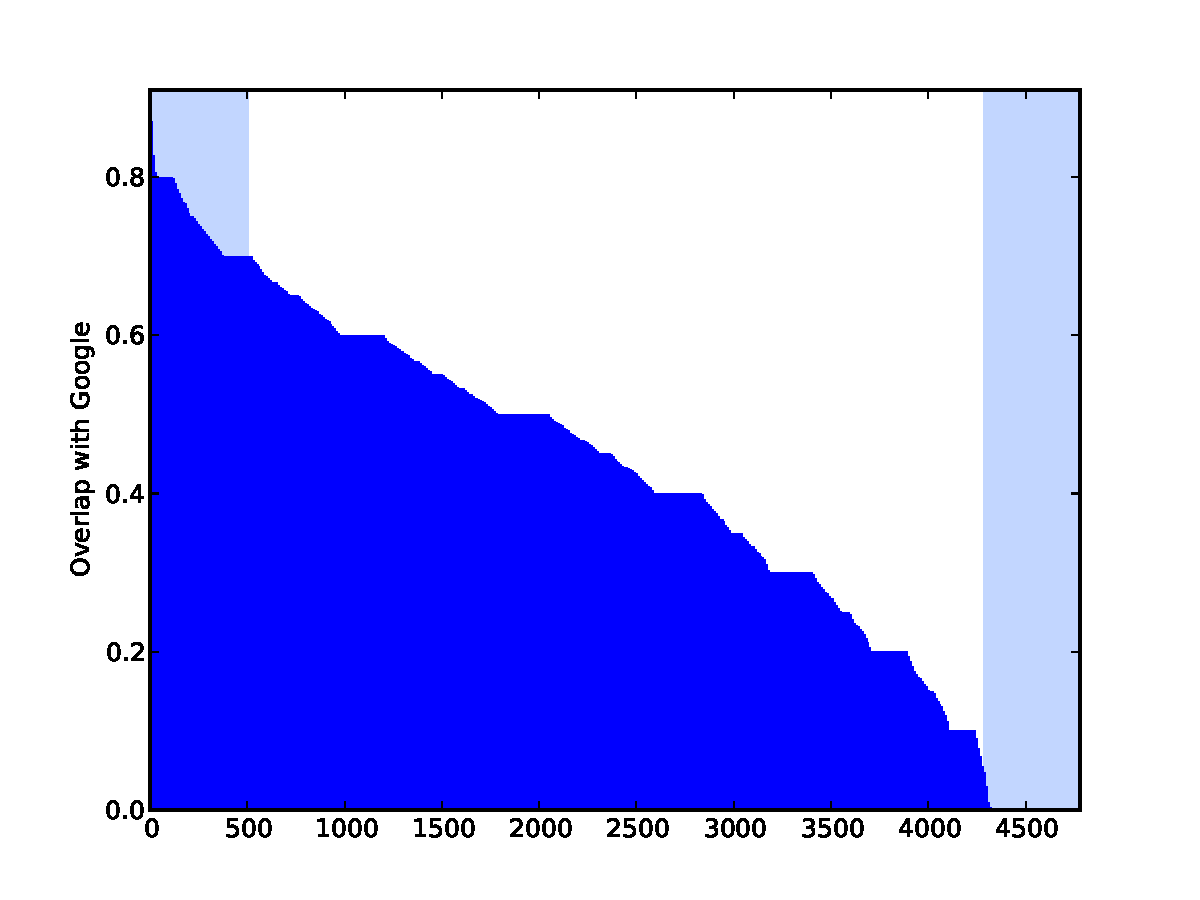
\includegraphics[width=\linewidth]{figures/turker-googmatch-distribution.pdf}
\caption{Individual turker overlap with Google Translate. We remove the 500 workers with the highest overlap (shaded region on left) from our analysis. Workers with no overlap (on right) are also likely to be cheating, e.g. by submitting random text. We target these workers through our embedded controls.}                
\label{dist}
\end{figure}

\begin{figure}[h]
\centering
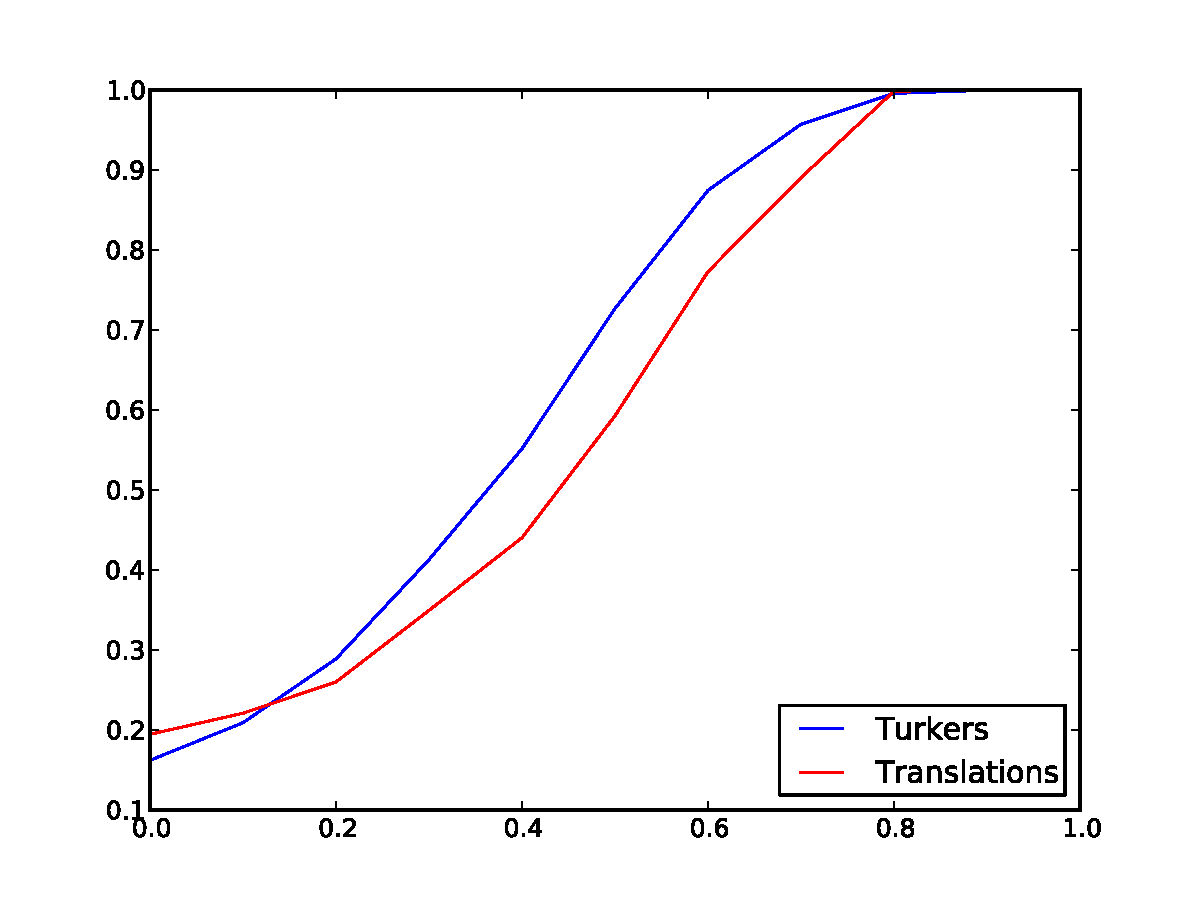
\includegraphics[width=\linewidth]{figures/google-cdf-googlangs.pdf}
\caption{Cumulative distribution of overlap with Google translate for workers and translations. Eliminating all workers with \textgreater 70\% overlap with google translate still preserves 90\% of translations and \textgreater 90\% of workers.}
\label{cdf}
\end{figure}

We have re-done our analysis to address this issue.  We compute the overlap between individual Turkers and Google translate (across all items, not just our controls).   Figure \ref{dist} plots the overlap, ranking from the Turker with the most overlap to the Turker with the least overlap.  To address the reviewers' concerns, we exclude the 500 Turkers with the highest overlap with Google translate, and remove them from all subsequent analyses in the paper.  This is equivalent to choosing a threshold value of approximately 70\% overlap, and excluding all Turkers whose translations overlap with Google at that rate or higher.  
Figure \ref{cdf} shows that removing workers at or above the 70\% threshold retains 90\% of the collected translations and over 90\% of the workers.

Our methodology now catches two types of cheating that can be done by Turkers who do not truly speak the language: 
\begin{enumerate}
\item Submitting random words -- detected by low accuracy on our gold standard controls.
\item Using online MT systems or dictionaries (approximated with Google Translate) -- detected by high overlap with Google on all items.
\end{enumerate}

This modification to our experimental design excludes the Indian workers who were producing good Afrikaans-English translations, which Reviewer F highlighted as problematic.  

Figure \ref{qual} shows how the overall quality estimates for each language have changed between the initial submission of the paper (top graph) and this revised version (bottom graph).

%\begin{figure}
%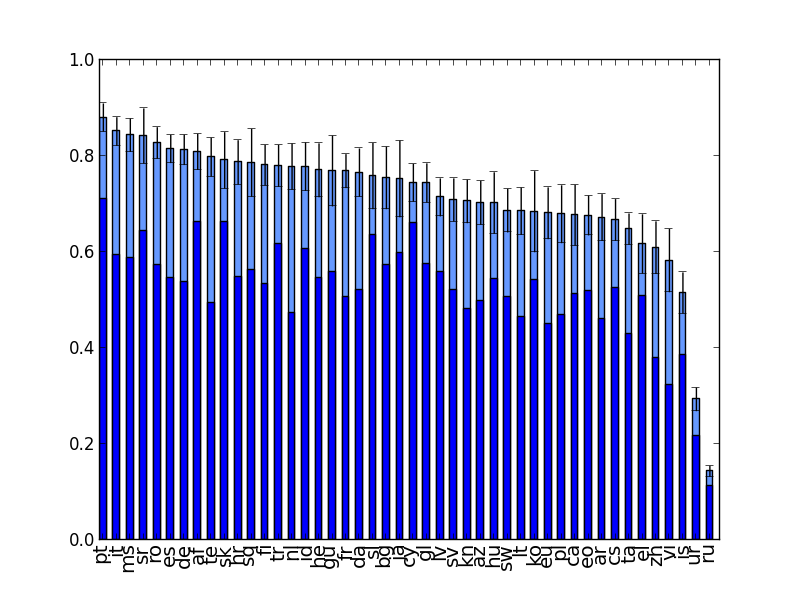
\includegraphics[width=\linewidth]{figures/quality-all.png}
%\caption{All turkers.}                
%\label{quality-all}
%\end{figure}
%\begin{figure}
%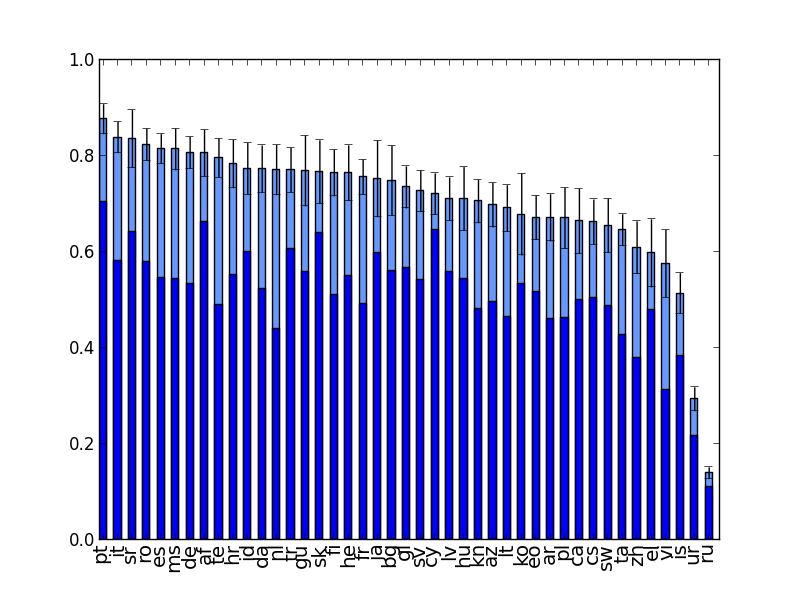
\includegraphics[width=\linewidth]{figures/quality-filtered.png}
%\caption{Turkers with \textless 70\% overlap with Google Translate.}
%\label{quality-filtered}
%\caption{Qualities for languages with \textgreater 50 turkers. Dark blue shows quality measured by perfect match on the control translation. Light blue indicates quality measured by included synonymous translations.}\label{qual}
%\end{figure}

Reviewer E also had an interesting suggestion on an alternate way that this problem could have been addressed:
\begin{quote}
This problem could have been avoided if the assignments were more suitable
for measuring real language proficiency. For example, unlike single-word
translations which can be solely conducted using a language resource,
phrase- or sentence-level translations are a more realistic indication of
the translator's knowledge of language. The challenge here would be to
devise the control set, i.e., to come up with gold standard translations of
such multi-word units. 
\end{quote}
At the outset of the study we considered asking workers to translate full sentences instead of individual words.  As the reviewer notes, it is quite challenging to find good controls for such a broad range of languages.  Ideally, we would have liked to have re-created Zaidan and Callison-Burch (2011)'s comparison of Turker translations of Urdu to professional translations, and applied it to 100 languages.   Unfortunately, finding a good set of test sentences for each language proved impossible.  While there are some documents which have been translated into all languages, like the Bible or the Universal Declaration of Human Rights, it is probable that Google already includes them in its training data. 

Instead of attempting all languages, and systematically comparing the quality of professionals against non-professionals, we create sentential translations for 6 languages, and train machine translation systems from the resulting parallel corpora.  This is described in section \ref{smt-results}.

\section{Are the results robust, or do a few big contributors dominate?}

The Action Editor and Reviewer G highlighted the possibility that the quality results are due to a few large players, and may not be robust if the experiment were rerun with a different group of workers: 
\begin{quote}
Provide additional analysis showing that translation accuracy is not due to a few individuals who happened to do most of your tasks.
\end{quote}

We agree that this is a valid concern since many languages followed the pattern of having a small number of very active Turkers complete the majority of assignments. In the new version of the paper, we account for this by defining our per-language accuracy as an average over {\it Turker qualities}, rather than over {\it assignment qualities}. With this method, each Turker contributes equally to the language's average quality, regardless of the number of HITs that that Turker submitted. Section 4 of the paper has been updated to reflect this change. 

Figure \ref{qual_dots} shows the quality scores for languages computed over assignments and over Turkers, and the change in each when the 10 most active Turkers in each language are removed. We can see that the per-Turker quality measure is robust to the exclusion of these highly-contributing Turkers. 

For completeness, we have also updated our reported quality scores in the paper to include confidence intervals and p-values, where appropriate. We hope this helps to reduce concern about the robustness of these measures.


\begin{figure}
\centering
\begin{subfigure}[b]{1\linewidth}
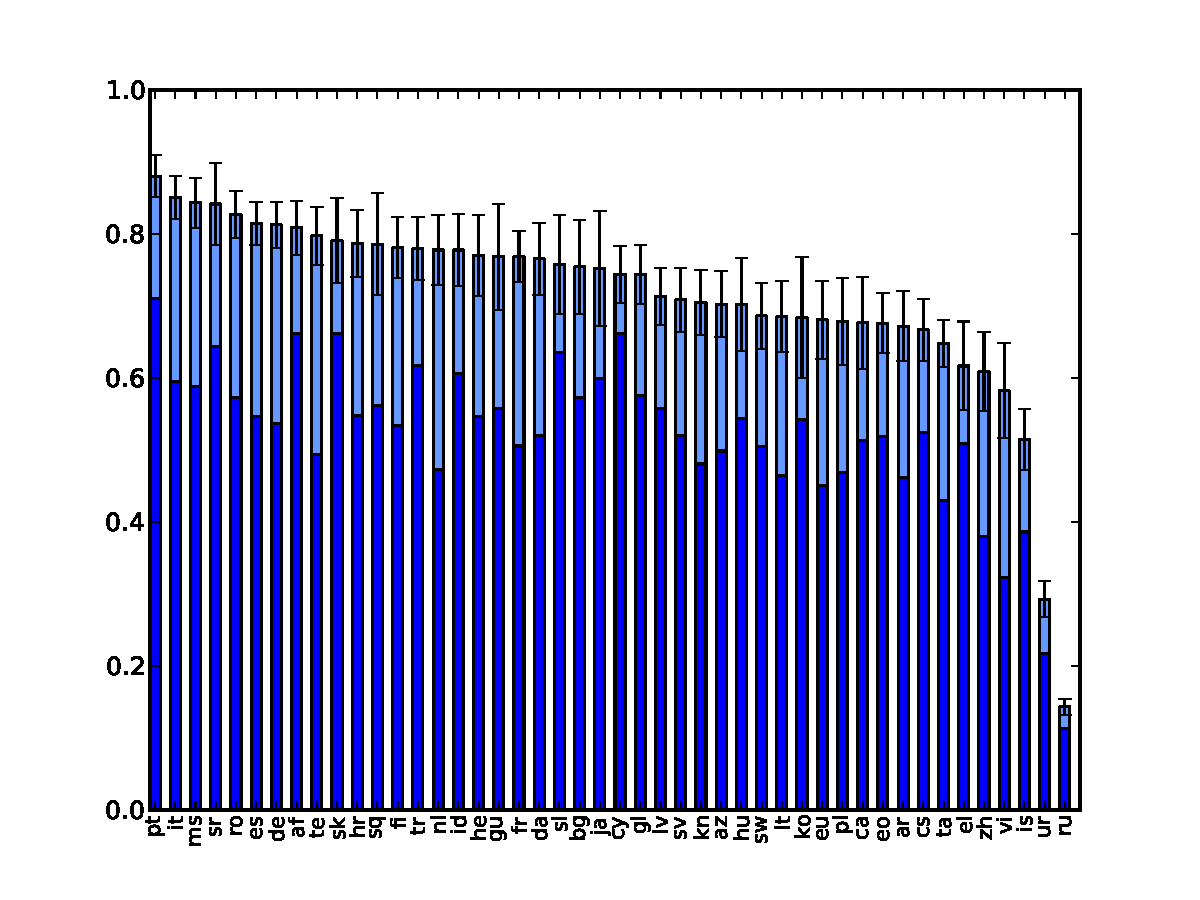
\includegraphics[width=\textwidth]{figures/quality-all.pdf}
\caption{All turkers.}                
\label{quality-all}
\end{subfigure}
\begin{subfigure}[b]{1\linewidth}
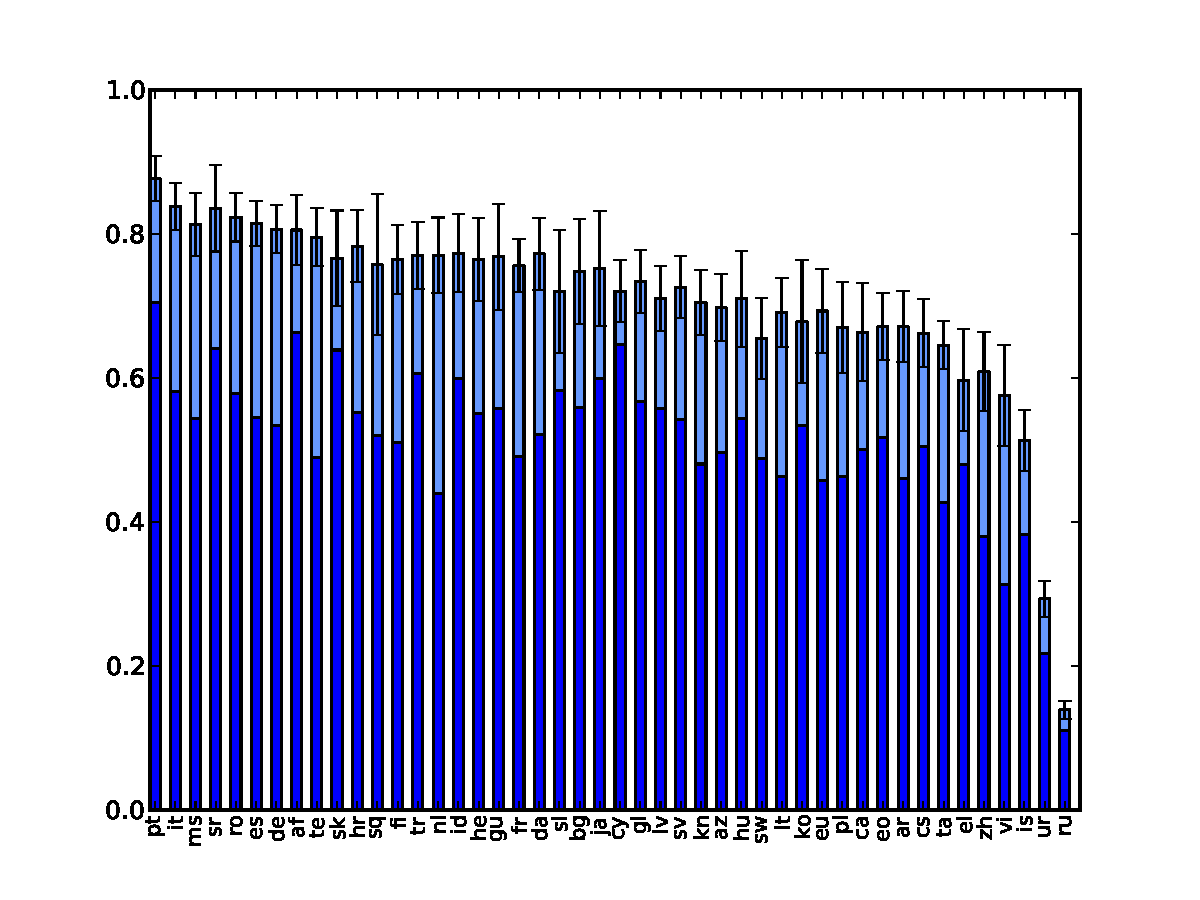
\includegraphics[width=\textwidth]{figures/quality-filtered.pdf}
\caption{Turkers with \textless 70\% overlap with Google Translate.}
\label{quality-filtered}
\end{subfigure}
\caption{Qualities for languages with \textgreater 50 turkers. Dark blue shows quality measured by perfect match on the control translation. Light blue indicates quality measured by included synonymous translations.}\label{qual}
\end{figure}


%\begin{figure}
%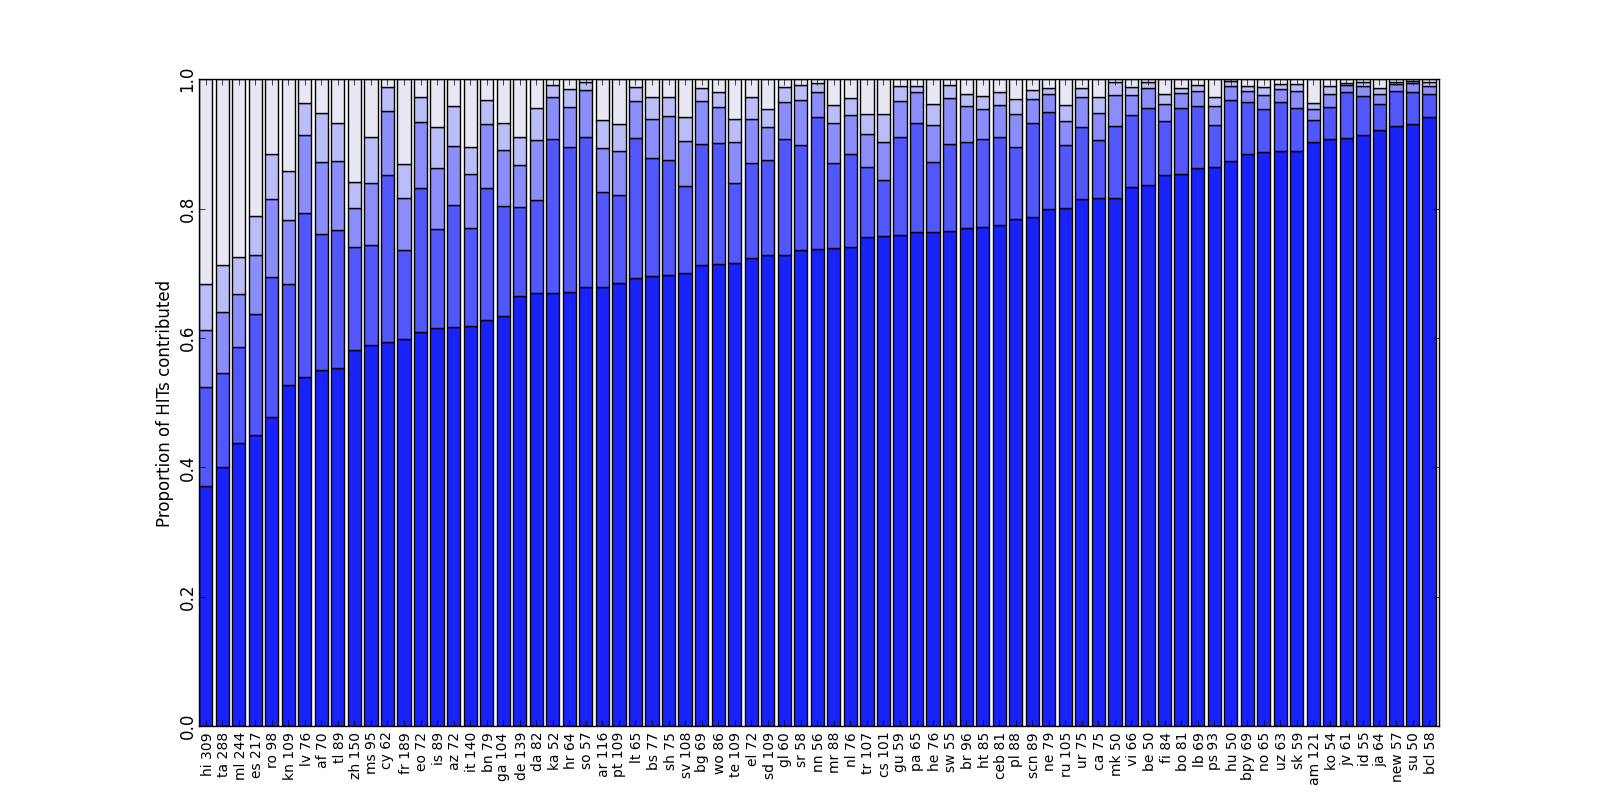
\includegraphics[height=1\linewidth, angle=270]{figures/turker-hit-contributions.png}
%\caption{Contributions of individual turkers to the overall number of HITs in each language. The dark blue bar represents the proportion of total HITs which were completed by the 10 highest-contributing turkers. The next darkest bar represents the next 10 highest-contributing turkers, and likewise for the thrid and forth darkest. The final bar represents the remaining turkers which were not one of the top 40 contributors.}
%\label{num./hits}
%\end{figure}

\section{Using crowdsourced data to train SMT systems, and evaluating the improvements due to dictionaries}\label{smt-results}

All the reviewers expressed desire for further evidence of the usefulness of the Turker-provided translations for statistical machine translation, and the possibility of extending the demonstrated methods to multiple word translations. 
To address these suggestions, we have added a new set of experiments to the paper.  In the new experiments, we collect full-sentence translations for six Indian languages which are well-represented on MTurk but for which there are currently no professionally-translated corpora available. We use the collected sentences to train and evaluate an SMT system, and show that the systems achieve decent performance. Furthermore, we add the collected single-word dictionaries to the training of these systems, and show that this produces measurable improvement in performance. Table \ref{dictionary_bleu} highlights these results. Please see sections 3 and 5 of the revised paper for a complete discussion of the data and experiments. 

{\bf NB: We previously published experiments using this Indian language data, but the work has only appeared in an ACL workshop paper and not in a main conference paper nor a journal article.  We hope that it is therefore allowable for inclusion here.}.   The workshop publication will be cited appropriately in the final version of the paper, but we omit the citation now so as not to de-anonymize the submission.   The analysis of the effect of the dictionaries on the SMT performance is new.


\begin{figure}
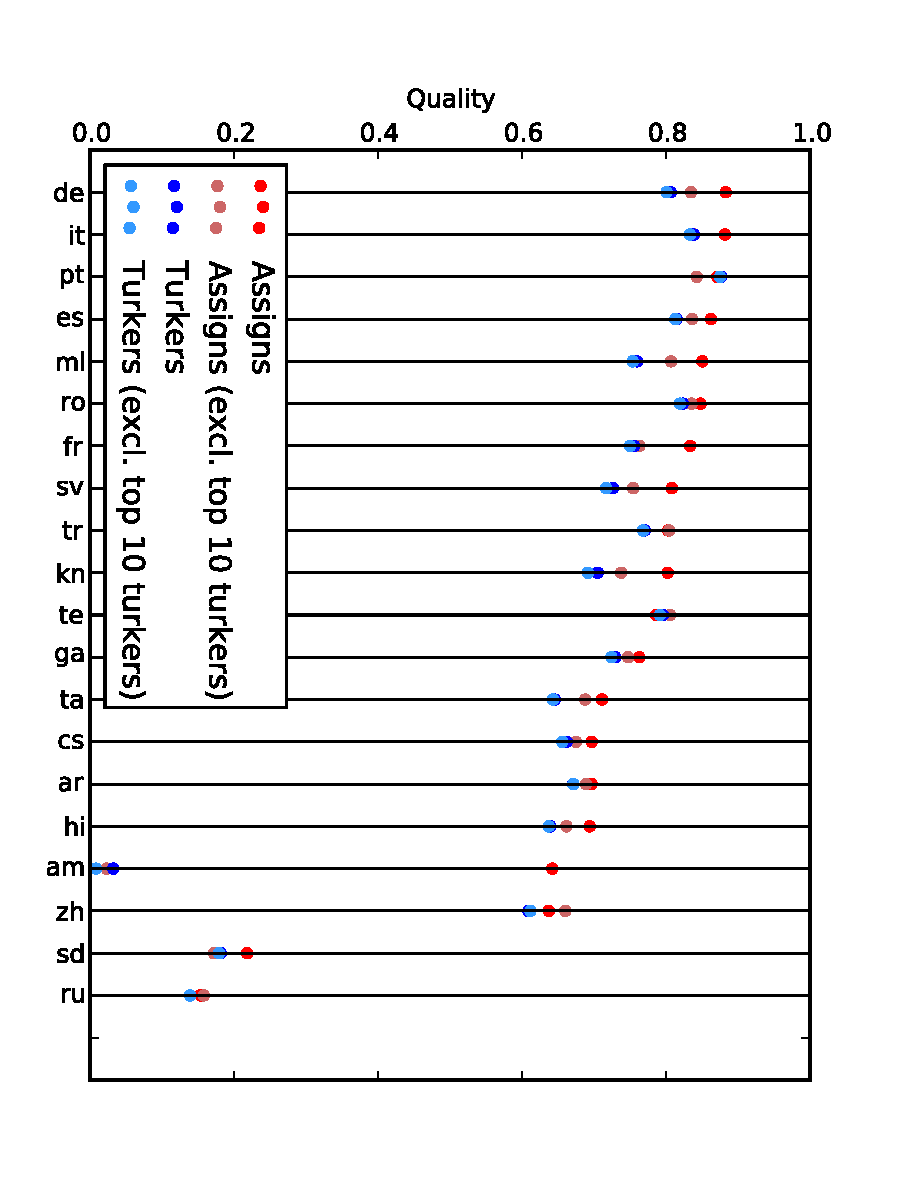
\includegraphics[width=1\linewidth]{figures/quality_compare.pdf}
\caption{Quality scores of languages computed as averages over assignments (red) and over turkers (blue). Light blue and light red dots reflect the quality scores that result when the 10 turkers with who contributed the highest number of HITs are removed. We see that while the quality calculated over assignments responds noticeably to the exclusion of these highly active turkers, the quality calculated over turkers is quite robust to the change.}
\label{qual_dots}
\end{figure}


\begin{table}[t]
\centering
\begin{tabular}{l|cc}
  language  & sentences &  dictionaries \\
  \hline\hline
  Bengali    &  12.03 & 17.29\\
  Hindi      & 16.19 & 18.10\\  
  Malayalam    &  6.65 & 9.72\\      
  Tamil      & 8.08 & 9.66 \\  
  Telugu     & 11.94 & 13.70\\  
  Urdu        & 19.22 & 21.98\\   
\end{tabular}
\caption{BLEU scores for translating into English using full sentence translations alone, and with the addition of single-word dictionaries. Scores are calculated using four reference translations and represent the mean of three MERT runs.}
\label{dictionary_bleu}
\end{table}

\section{Other suggestions: Does time of day that HIT was posted change the outcome?}

Reviewer F raised a question about the relation between time of day and Turker activity: 

\begin{quote}
Did the authors take into account time of day, when the HIT was posted etc. to get a sense of whether one time of day is more optimal than others for each language? Does it matter at all?
\end{quote}
Figure \ref{time} shows the activity over a 24 hour day for 23 languages with greater than 100 turkers each. The plot shows that activity does vary across time zones, and suggests that choosing the release time intelligently based on the HIT language is likely to affect how quickly it is completed. We include this analysis here for the interest of the reviewer. We do not include it in the paper, however, as we do not feel it meaningfully changes the analysis presented there. 

\begin{figure}
\centering
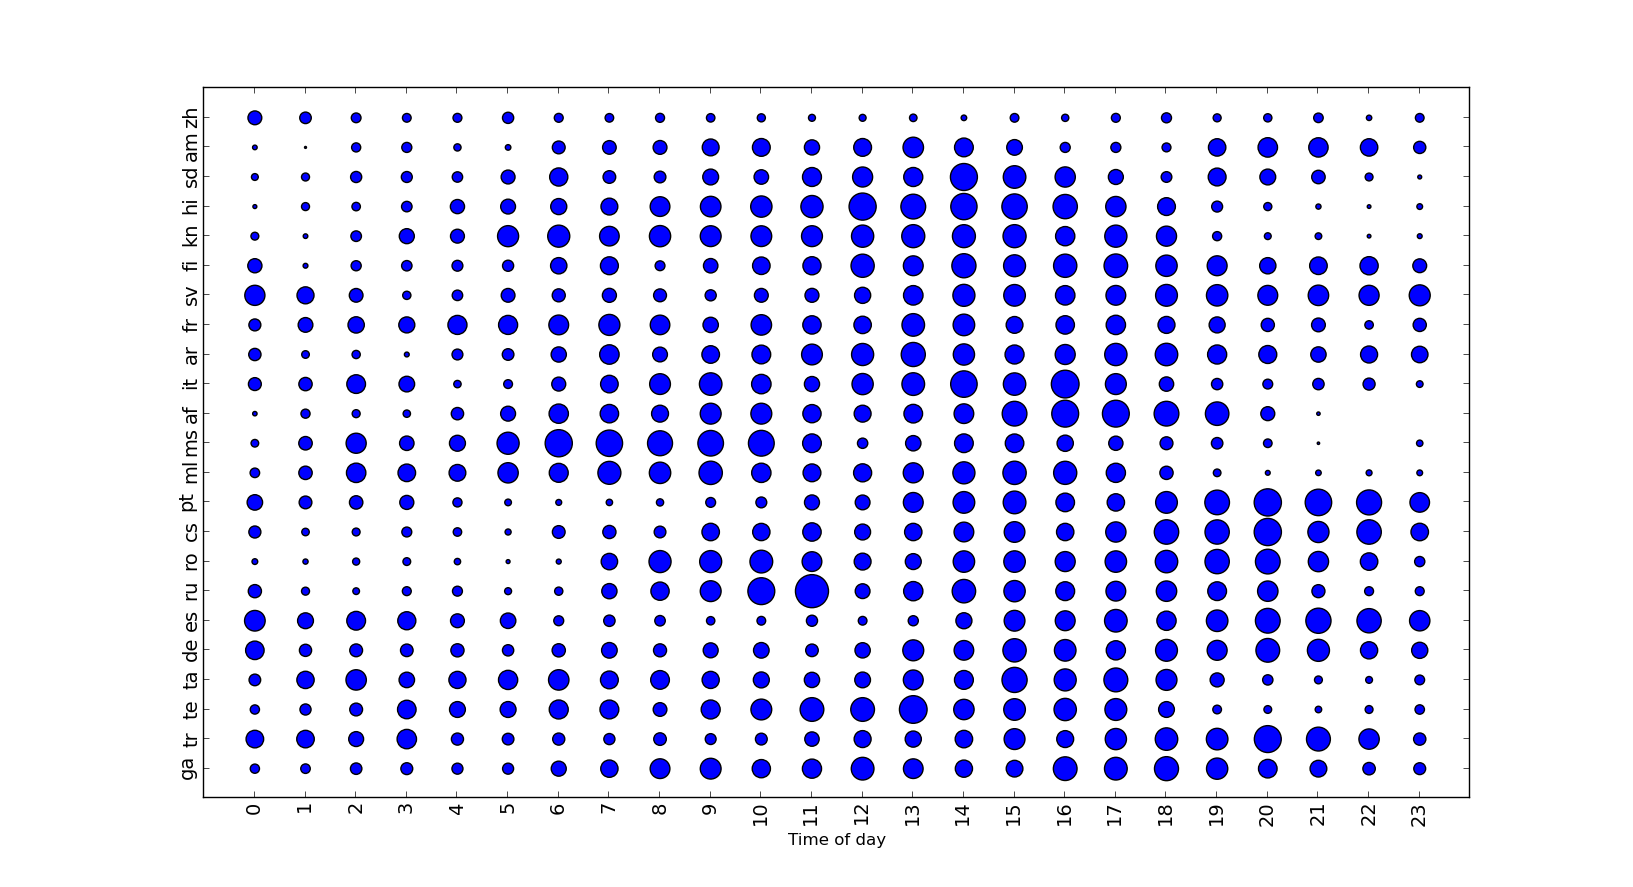
\includegraphics[height=.8\linewidth, angle=270]{figures/times.png}
\caption{Number of HITs completed during each hour of the day for languages with \textgreater 100 turkers.}
\label{time}
\end{figure}

\section{Other suggestions: longitudinal study. }

 Reviewer B asked: 
\begin{quote}
The authors ran an experiment over 3.5 months, but I wonder how the demographics change over time. Are there seasonal effects in the workforce? Has it changed over the past year? And more importantly, will it change substantially in the future? I'm somewhat skeptical that these demographics will remain constant, especially as Amazon rolls out changes to the service.
\end{quote}

While we agree that the questions posed are very interesting, we feel that answering these questions is the subject of another study. It is true that the current demographic makeup of MTurk workers is likely to shift, but we cannot currently take on the expense of conducting a long term study (the study presented here cost more than \$40K). We have updated the text of the paper to emphasize this limitation in our results by adding the following sentences to our Discussion section: 
\begin{quote}
The demographics reported in this study are likely to shift over time. Amazon may change its expand its payments to new currencies.  Posting long-running HITs in other languages may recruit more speakers of those languages.  New crowdsourcing platforms may emerge. The data presented here provides a valuable snapshot of the current state of MTurk, and the methods used can be applied generally in future research.
\end{quote}

\section{Other suggestion: Accuracy of Geolocation}

Reviewers B and E were concerned about the accuracy of geolocation. 
We understand that geolocation is not perfect, which is why we propose the use of location data as just one of several criteria by which to identify likely qualified translators. The trends that we observe in our analysis, where we show that turkers geolocated within a region likely to speak the source language being translated tend to perform better on our controls, coincide with what we would expect to see if geolcation were accurate. Additionally, of the turkers who responded to our survey questions, 95\% of their self-reported locations agreed with our geolocations. These facts reassure us that, on average, the geolocation is performing sufficiently well.

\section{Other suggestions: specific recommendations}

Reviewer F said:
\begin{quote}
I was a little disappointed that the paper does not provide more specific
recommendations for low-resource languages.
\end{quote}

We have strengthened the conclusions to be more clear.  We have included a table that shows what languages are currently good for researchers to target based on the size of the speaker populations, the quality of the translations, and how fast the translations were completed.  Table \ref{recommendations} now appears in the Discussion section of the revised submission. 


%%%%%%%%%%%%%%%%%%%%%%%%%%
\begin{table}
\centering
\footnotesize
\small
\begin{tabular}{|p{.1\linewidth}|p{.1\linewidth}|p{.1\linewidth}|p{0.5\linewidth}|}
\hline
\footnotesize workers & \footnotesize  quality & \footnotesize speed & \\\hline
%many &high&fast&\cellcolor[rgb]{0.5, 0.8, 0.5} de es fr gu it kn ml nl pt ro sr te tl \\\cline{3-4}
%&&slow& ar ga he pa sv tr\\\cline{2-4}
%& low or medium &fast& hi mr ta ur \\\cline{3-4}
%&&slow&bn bo bpy ceb ne new pl ru sd zh\\\cline{1-4}
many &high&fast&\cellcolor[rgb]{0.5, 0.8, 0.5}    Dutch, French, German, Gujarati, Italian, Kannada, Malayalam, Portuguese, Romanian, Serbian, Spanish, Tagalog, Telugu \\\cline{3-4}
&&slow& Arabic,  Hebrew, Irish, Punjabi, Swedish, Turkish\\\cline{2-4}
& low   &fast& Hindi, Marathi, Tamil, Urdu \\\cline{3-4}
&or medium&slow&Bengali,  Bishnupriya Manipuri, Cebuano,  Chinese, Nepali, Newar, Polish, Russian, Sindhi, Tibetan\\\cline{1-4}
few &high  &fast& Bosnia, Croatian  Macedonian  Malay  Serbo-Croatian\\\cline{3-4}
&&slow&Afrikaans, Albanian, Aragonese, Asturian, Basque, Belarusian, Bulgarian, Central Bicolano, Czech, Danish, Finnish, Galacian, Greek, Haitian, Hungarian, Icelandic, Ilokano, Indonesian, Japanese, Javanese, Kapampangan, Kazakh, Korean, Lithuanian, Low Saxon, Malagasy, Norwegian (Bokmal), Sicilian, Slovak, Slovenian, Thai, Ukranian, Uzbek, Waray-Waray, West Frisian, Yoruba\\\cline{2-4}
&low   &fast&--\\\cline{3-4}
&or medium&slow&\cellcolor[rgb]{0.8, 0.5, 0.5}Amharic,  Armenian, Azerbaijani, Breton, Catalan, Georgian, Latvian, Luxembourgish, Neapolitian, Norwegian (Nynorsk), Pashto, Piedmontese, Somali, Sudanese, Swahili, Tatar, Vietnamese, Walloon, Welsh \\\hline
none&low or medium&slow&\cellcolor[rgb]{0.8, 0.5, 0.5}  Esperanto, Ido, Kurdish, Persian, Quechua, Wolof, Zazaki\\\hline
\end{tabular}
\normalsize
\caption{The green box shows the best languages to target on MTurk. These languages have many workers who generate high quality results quickly. We defined {\it many} workers as 50 or more active in-region workers, {\it high} quality as $\geq$70\% accuracy on the gold standard controls, and {\it fast} if all of the 10,000 words were completed within two weeks.}
\label{recommendations}
\end{table}
%%%%%%%%%%%%%%%%%%%%%%%%%%%%%%%%%%%%%%%


\end{document}
